\documentclass[conference]{IEEEtran}
\IEEEoverridecommandlockouts
% The preceding line is only needed to identify funding in the first footnote. If that is unneeded, please comment it out.

\usepackage[english]{babel}
\usepackage{amsthm}
\usepackage{cite}
\usepackage{amsmath,amssymb,amsfonts}
\usepackage{algorithmic}
\usepackage{graphicx}
\usepackage{textcomp}
\usepackage{xcolor}
\usepackage[a4paper, total={184mm,239mm}]{geometry}
\def\BibTeX{{\rm B\kern-.05em{\sc i\kern-.025em b}\kern-.08em
    T\kern-.1667em\lower.7ex\hbox{E}\kern-.125emX}}

\theoremstyle{definition}
\newtheorem{definition}{Definition}

\usepackage{listings}
\usepackage{stfloats}
\usepackage{graphicx}
\usepackage{caption}
\usepackage{xcolor}
% \usepackage[fleqn]{amsmath}
\usepackage{lstautogobble}  % Fix relative indenting
\usepackage{color}          % Code coloring
\usepackage{zi4}            % Nice font

\definecolor{bluekeywords}{rgb}{0.13, 0.13, 1}
\definecolor{graycomments}{rgb}{0.5, 0.5, 0.5}
\definecolor{redstrings}{rgb}{0.9, 0, 0}
\definecolor{graynumbers}{rgb}{0.5, 0.5, 0.5}

\lstset{
    autogobble,
    columns=fullflexible,
    showspaces=false,
    showtabs=false,
    breaklines=true,
    showstringspaces=false,
    breakatwhitespace=true,
    escapeinside={(*@}{@*)},
    commentstyle=\color{graycomments},
    keywordstyle=\color{bluekeywords},
    stringstyle=\color{redstrings},
    numberstyle=\color{graynumbers},
    basicstyle=\ttfamily,
    xleftmargin=18pt,
    xrightmargin=2pt,
    tabsize=4,
    captionpos=b
}
\lstset
{ %Formatting for code in appendix
    language=Matlab,
    % basicstyle=\footnotesize,
    numbers=left,
    stepnumber=1,
    showstringspaces=false,
    tabsize=1,
    breaklines=true,
    breakatwhitespace=false,
}
\lstset{
numbers=left, 
numberstyle=\small, 
numbersep=8pt, 
frame = single, 
language=Pascal, 
framexleftmargin=15pt}

\pagestyle{empty}
\begin{document}

\title{ChiselFV: A Formal Verification Framework for Chisel
% {\footnotesize \textsuperscript{*}Note: Sub-titles are not captured in Xplore and
% should not be used}
% \thanks{Identify applicable funding agency here. If none, delete this.}
}


\maketitle

% 现代硬件设计越来越复杂 -> 敏捷开发技术 -> Chisel -> Formal for Chisel -> ChiselFV
\begin{abstract}
    Modern digital hardware is becoming ever more complex. And agile development, an efficient idea in software development, has been introduced into hardware. Furthermore, as a new hardware construction language, Chisel helps to raise the level of hardware design abstraction with the support of object-oriented and functional programming. Chisel plays a crucial role in future hardware design and open-source hardware development. However, the formal verification for Chisel is still limited. In this paper, we propose ChiselFV, a formal verification framework that has supported detailed formal hardware property descriptions and integrated mature formal hardware verification flows based on SymbiYosys. It builds on top of Chisel and uses Scala to drive the verification process. Thus the framework can be seen as an extension of Chisel. ChiselFV makes it easy to verify hardware designs formally when implementing them in Chisel.
\end{abstract}

\begin{IEEEkeywords}
    Hardware verification, Formal methods, Hardware description language, Chisel
\end{IEEEkeywords}

\section{Introduction}
% 硬件设计需求复杂,Chisel 出现,Chisel 优势
Over the past several years, hardware design has grown to be ever more and more complex. The increased demand for high-performance computing systems has led to a larger need for domain-specific hardware accelerators \cite{dally2020domain}.
The dominant traditional hardware description languages (HDLs), Verilog and VHDL, were initially developed as hardware simulation languages and were only later adopted as a basis for hardware synthesis. So these languages lack the powerful abstraction facilities that are common in modern software languages, which leads to low productivity because it is difficult to reuse components.
Chisel \cite{bachrach2012chisel}, a Scala-embedded hardware construction language, was introduced in order to lift digital circuit description to a more software-like high-level language \cite{dobis2021chiselverify}.
Chisel attempts to solve these problems by providing functional and object-oriented programming support. With these features, Chisel supports advanced hardware design using highly parameterized generators and improves the abstraction level of hardware design. However, Chisel lacks the powerful and easy-to-use formal verification support that is mature in traditional HDLs.

% 硬件验证必要性,Chisel 上的形式化验证工作不足 + 无法直接迁移
In hardware development, because of the high cost of trial and error, verifying the correctness of the design is essential, especially for trusted systems which are constantly dealing with human lives or may cause a massive loss if an unexpected event occurs. Therefore, we need to use many test cases to simulate the design to find bugs and use formal methods to ensure correctness. There are many mature verification methods in traditional hardware languages. However, in Chisel, the work of formal verification is still limited, and the previous workflow for low level RTL cannot be migrated to Chisel easily.

% Chisel 上的验证工作:ChiselVerify + 官方的 Chisel Formal 支持。相比成熟的 HDLs 的形式化支持,这些都是比较原始的。 
Currently, there is some work on the Chisel level to verify the correctness of the design. ChiselVerify is a verification framework inspired by Universal Verification Method(UVM) \cite{mehta2018uvm} and implemented on the Chisel level and supports both coverage-oriented and constrained random verification (CRV) flows \cite{dobis2021chiselverify}. However, ChiselVerify only focuses on applying software testing techniques to hardware verification.
Recently, Berkeley provided Chisel developers with an easy way to formally verify the designs \cite{dobis2021open}. They added a formal backend to the FIRRTL compiler, which converts a high-level intermediate representation (IR) into a normalized structural representation. The backend can translate FIRRTL expressions to the bit-vector expression language defined by the SMTLib format \cite{barrett2010smt}, and then use the Z3 solver \cite{moura2008z3} to execute the Bounded Model Checking (BMC) algorithm \cite{biere2009bounded}.
% 然而目前它支持的性质描述十分有限,仅支持对返回为 Boolean 类型值的表达式断言,而且支持的验证方法也只有 BMC。和现有的低层次 HDL 的形式化支持相比,它显得十分初级。
However, the current support for property description is very limited. It only supports assertions on expressions that return Boolean values, and the verification algorithm it supports is only BMC. Compared with the existing formal support for other HDLs, they are very primitive.

% 传统 HDLs 中的方案中,SVA 描述强大,验证方案丰富。但是迁移有问题:生成的代码可读性差,参数化。
% 在传统的硬件设计语言中,有着成熟的硬件验证技术支持,但是无法直接迁移到 Chisel 中。
Traditional HDLs have mature hardware verification techniques, but they cannot be directly migrated to Chisel.
% 例如,可以使用 SystemVerilog Assertions(SVA)来描述性质。它支持复杂的时序性质描述。它可以和 SystemVerilog 代码一起被 Yosys 工具综合,转化为迁移系统,使用 SAT / SMT 求解器为基础的各种模型检测算法求解。
For example, SystemVerilog Assertions (SVA) \cite{vijayaraghavan2005practical} can be used to describe properties. SVA is a essentially a language construct which provides a powerful way to write constraints, checkers, and cover points for hardware designs. It supports complex temporal property descriptions. It can be synthesized with SystemVerilog code by Yosys \cite{wolf2016yosys} and converted to a transition system, which can be solved by various model checking algorithms based on SAT/SMT solvers.
% 目前 Chisel 语言主要用于在高层构造硬件生成器,然后生成 SystemVerilog 代码用于综合。在生成 SystemVerilog 中定义性质描述时不可行的,一方面生成的 SystemVerilog 代码可读性很差,设计复杂时,很难找到 Chisel 中对应的信号,因此很难在这里添加性质描述;同时,Chisel 的优势在于高度参数化,但是在 SystemVerilog 层次已经完成了 Chisel 模块的实例化,因此需要在每次实例化时重新定义性质,这是不可取的。
Currently, Chisel is mainly used to construct hardware generators at the high level and then generate SystemVerilog code for synthesis. It is not feasible to define property descriptions in SystemVerilog, because the generated SystemVerilog code is difficult to read, making it hard to find the corresponding signals in Chisel when the design is complex. In addition, Chisel's advantage is high parameterization, but in the generated SystemVerilog, the module instantiation has been completed, so the property needs to be redefined every time the module is instantiated, which is not desirable.

% 所以我们的工作就是把传统 HDLs 中的验证能力在 Chisel 层次进行实现
% 因此我们选择直接在 Chisel 上进行性质定义,并且致力于使 Chisel 具有和传统 HDLs 相同能力的形式化支持。
Therefore, we choose to define properties directly on Chisel and strive to make Chisel have the same formal support as traditional HDLs. 
Our main contribution in this paper is to propose ChiselFV, a formal verification framework for Chisel, which can be found in the GitHub repository \cite{ChiselFV}.
We also provide the workflow of formal verification on the Chisel level and detailed application of ChiselFV on the actual case. The contribution of this work is as follows:

\begin{itemize}
    \item \textbf{ChiselFV.} We propose a formal verification framework for Chisel, which can be used to describe hardware properties on the Chisel level. And we integrated the verification algorithm engine to perform verification in one-click. At the same time, our ChiselFV has the ability to describe the temporal properties and the ability to describe the free constant definition, which greatly enhanced the hardware properties description capability.
    \item \textbf{High-efficiency verification flow.} We propose a hardware verification workflow based on ChiselFV. With ChiselFV, we can synchronize the hardware properties description with the agile development process, thereby avoiding the design of complicated hardware properties in the low-level hardware. The hardware verification flow can be integrated into the agile hardware development process seaminglessly. 
    % 我们用多端口内存的正确性验证和一个教科书上的五级流水线设计验证来说明这点。
    We use the formal verification process of a multi-ported memory and a textbook five-stage pipeline design to illustrate this point.
\end{itemize}

This paper is organized into five sections. Section II uses Memory's example to explain the apparent advantages of formal verification on the Chisel level. Section III details ChiselFV and the workflow of formal verification on Chisel modules. Section IV describes how to verify multi-ported Memory using ChiselFV. Related work is in Section V. Section VI concludes.

\section{A Motivating Example}
In this section, we use a case to demonstrate the advantages of formal verification on the Chisel level.

% 内存是硬件中重要的一个部分,在 Chisel 中,提供了直接构造内存的库,从而使得我们可以很方便地得到一个参数化大小和位宽的内存模块。
Memory is an important part of hardware development, and Chisel provides a library to construct Memory directly, making it easy to get a memory module with a parameterized size and width.
% 可以看到,我们使用 15 行代码得到参数化内存。
We can quickly use 15 lines to get a parameterized memory in Chisel.

\begin{lstlisting}[language=scala, caption={A memory of size c and width w in Chisel}, label=mem]
class Memory(c: Int, w: Int) extends Module {
    val nw = log2Ceil(c)
    val io = IO(new Bundle {
        val wrEna = Input(Bool())
        val wrData = Input(UInt(w.W))
        val wrAddr = Input(UInt(nw.W))
        val rdAddr = Input(UInt(nw.W))
        val rdData = Output(UInt(w.W))
    })
    val mem = Mem(c, UInt(w.W))
    when(io.wrEna) {
        mem.write(io.wrAddr, io.wrData)
    }
    io.rdData := mem.read(io.rdAddr)
}
\end{lstlisting}

As shown in Listing \ref{mem}, this is a parameterized memory implemented in Chisel. The module has two constructor parameters, \verb|c| and \verb|w|, where \verb|c| is the size of the Memory, and \verb|w| is the width of the data in the Memory. We define the IO of the module (line 3-9), Memory (line 10), and read / write access  (line 11-14). It is easy to construct such a parameterized module in Chisel, but it is hard in SystemVerilog to define a resizeable memory module.

Next, we need to verify the correctness of the memory module. First, we need to describe the properties of the memory module in non-formal language: At any time, any address can write data, and after any time, if no write operation is performed on the address, the data read from the address should be the data written before. Then we need to convert the properties to a formal expression and package it with the memory module.
% 然而在当前的 Chisel 的形式化描述支持中,无法将上面的性质定义出来,因为这里需要一个定义一个任意值来描述地址或数据。
However, in the current Chisel formal support, the above properties cannot be defined, because here we need to define an arbitrary value to describe the address or data.

% 我们可以试着在 Chisel 上设计模块,然后在生成的 SystemVerilog 代码上进行形式化验证。
We can try to design the module on Chisel and then perform formal verification on the generated SystemVerilog code.
% Chisel 模块可以很容易生成对应的 SystemVerilog 代码,例如可以使用 Listing 2 中的代码块来实例化一个 1KB 的 Memory 模块。
Chisel modules can easily generate corresponding SystemVerilog code. For example, we can use the code in Listing \ref{initializememory} to instantiate a 1KB Memory module.

\begin{lstlisting}[language=Scala, caption={A Chisel code fragment using to instantiate 1KB Memory module in SystemVerilog}, label={initializememory}]
chisel3.stage.ChiselStage.emitSystemVerilog(new Memory(1024, 8))
\end{lstlisting}

% 然而,利用 Chisel 生成的低层次 RTL 进行形式化验证是繁琐且几乎不可行的。
However, using the low-level RTL generated by Chisel to perform formal verification is tedious and almost impossible. 
% 首先,Chisel 生成的低层次 RTL 可读性十分差。15 行的 Chisel 代码实例化得到的 SystemVerilog 代码有 80 行。同时如 Listing 3 所示的,生成的 SystemVerilog 中的变量名会被污染。Chisel 的编译过程是不去考虑生成电路的可读性的,因此在生成的低层次 RTL 中分析验证是不可取的。
First, the readability of the low-level RTL generated by Chisel is poor. The 15-line Chicodesode generates 80 lines of SystemVerilog code. As shown in Listing \ref{svcode}, the variable names in the generated SystemVerilog are polluted. Chisel's compilation process does not consider the readability of the generated circuit, so it is not appropriate to analyze and verify the generated low-level RTL.
% 其次,对于生成的 SystemVerilog 内存模块,其大小和宽度都确定了,不能参数化地定义性质,所以当参数发生变化了,我们需要重新编写性质描述来验证,这是低效率的。
Second, for the generated SystemVerilog memory module, its size and width are fixed, so we cannot parameterize the properties. When the parameters change, we need to rewrite the property description to verify it, which is inefficient. 

\begin{lstlisting}[language=Verilog, caption={A SystemVerilog code fragment generated by Chisel}, label={svcode}]
...
assign mem_MPORT_en = io_wrEna;
assign io_rdData = mem_io_rdData_MPORT_data; // @[Memory.scala 19:13]
always @(posedge clock) begin
    if (mem_MPORT_en & mem_MPORT_mask) begin
    mem[mem_MPORT_addr] <= mem_MPORT_data; // @[Memory.scala 14:16]
    end
end
...
\end{lstlisting}

\section{Formal Verification in Chisel}

This section gives the structure of ChiselFV, details the property description and algorithm engine support in ChiselFV and the methodology to perform formal verification on Chisel using ChiselFV.

\subsection{Framework Structure}

ChiselFV is based on Chisel and can be seen as an extension of formal verification in Chisel. The primary implementation uses Scala and enables Chisel modules to provide property descriptions and formal verification. The figure Fig \ref{fig: structure} shows the structure of ChiselFV.

\begin{figure}[!htbp]
    \begin{center}
    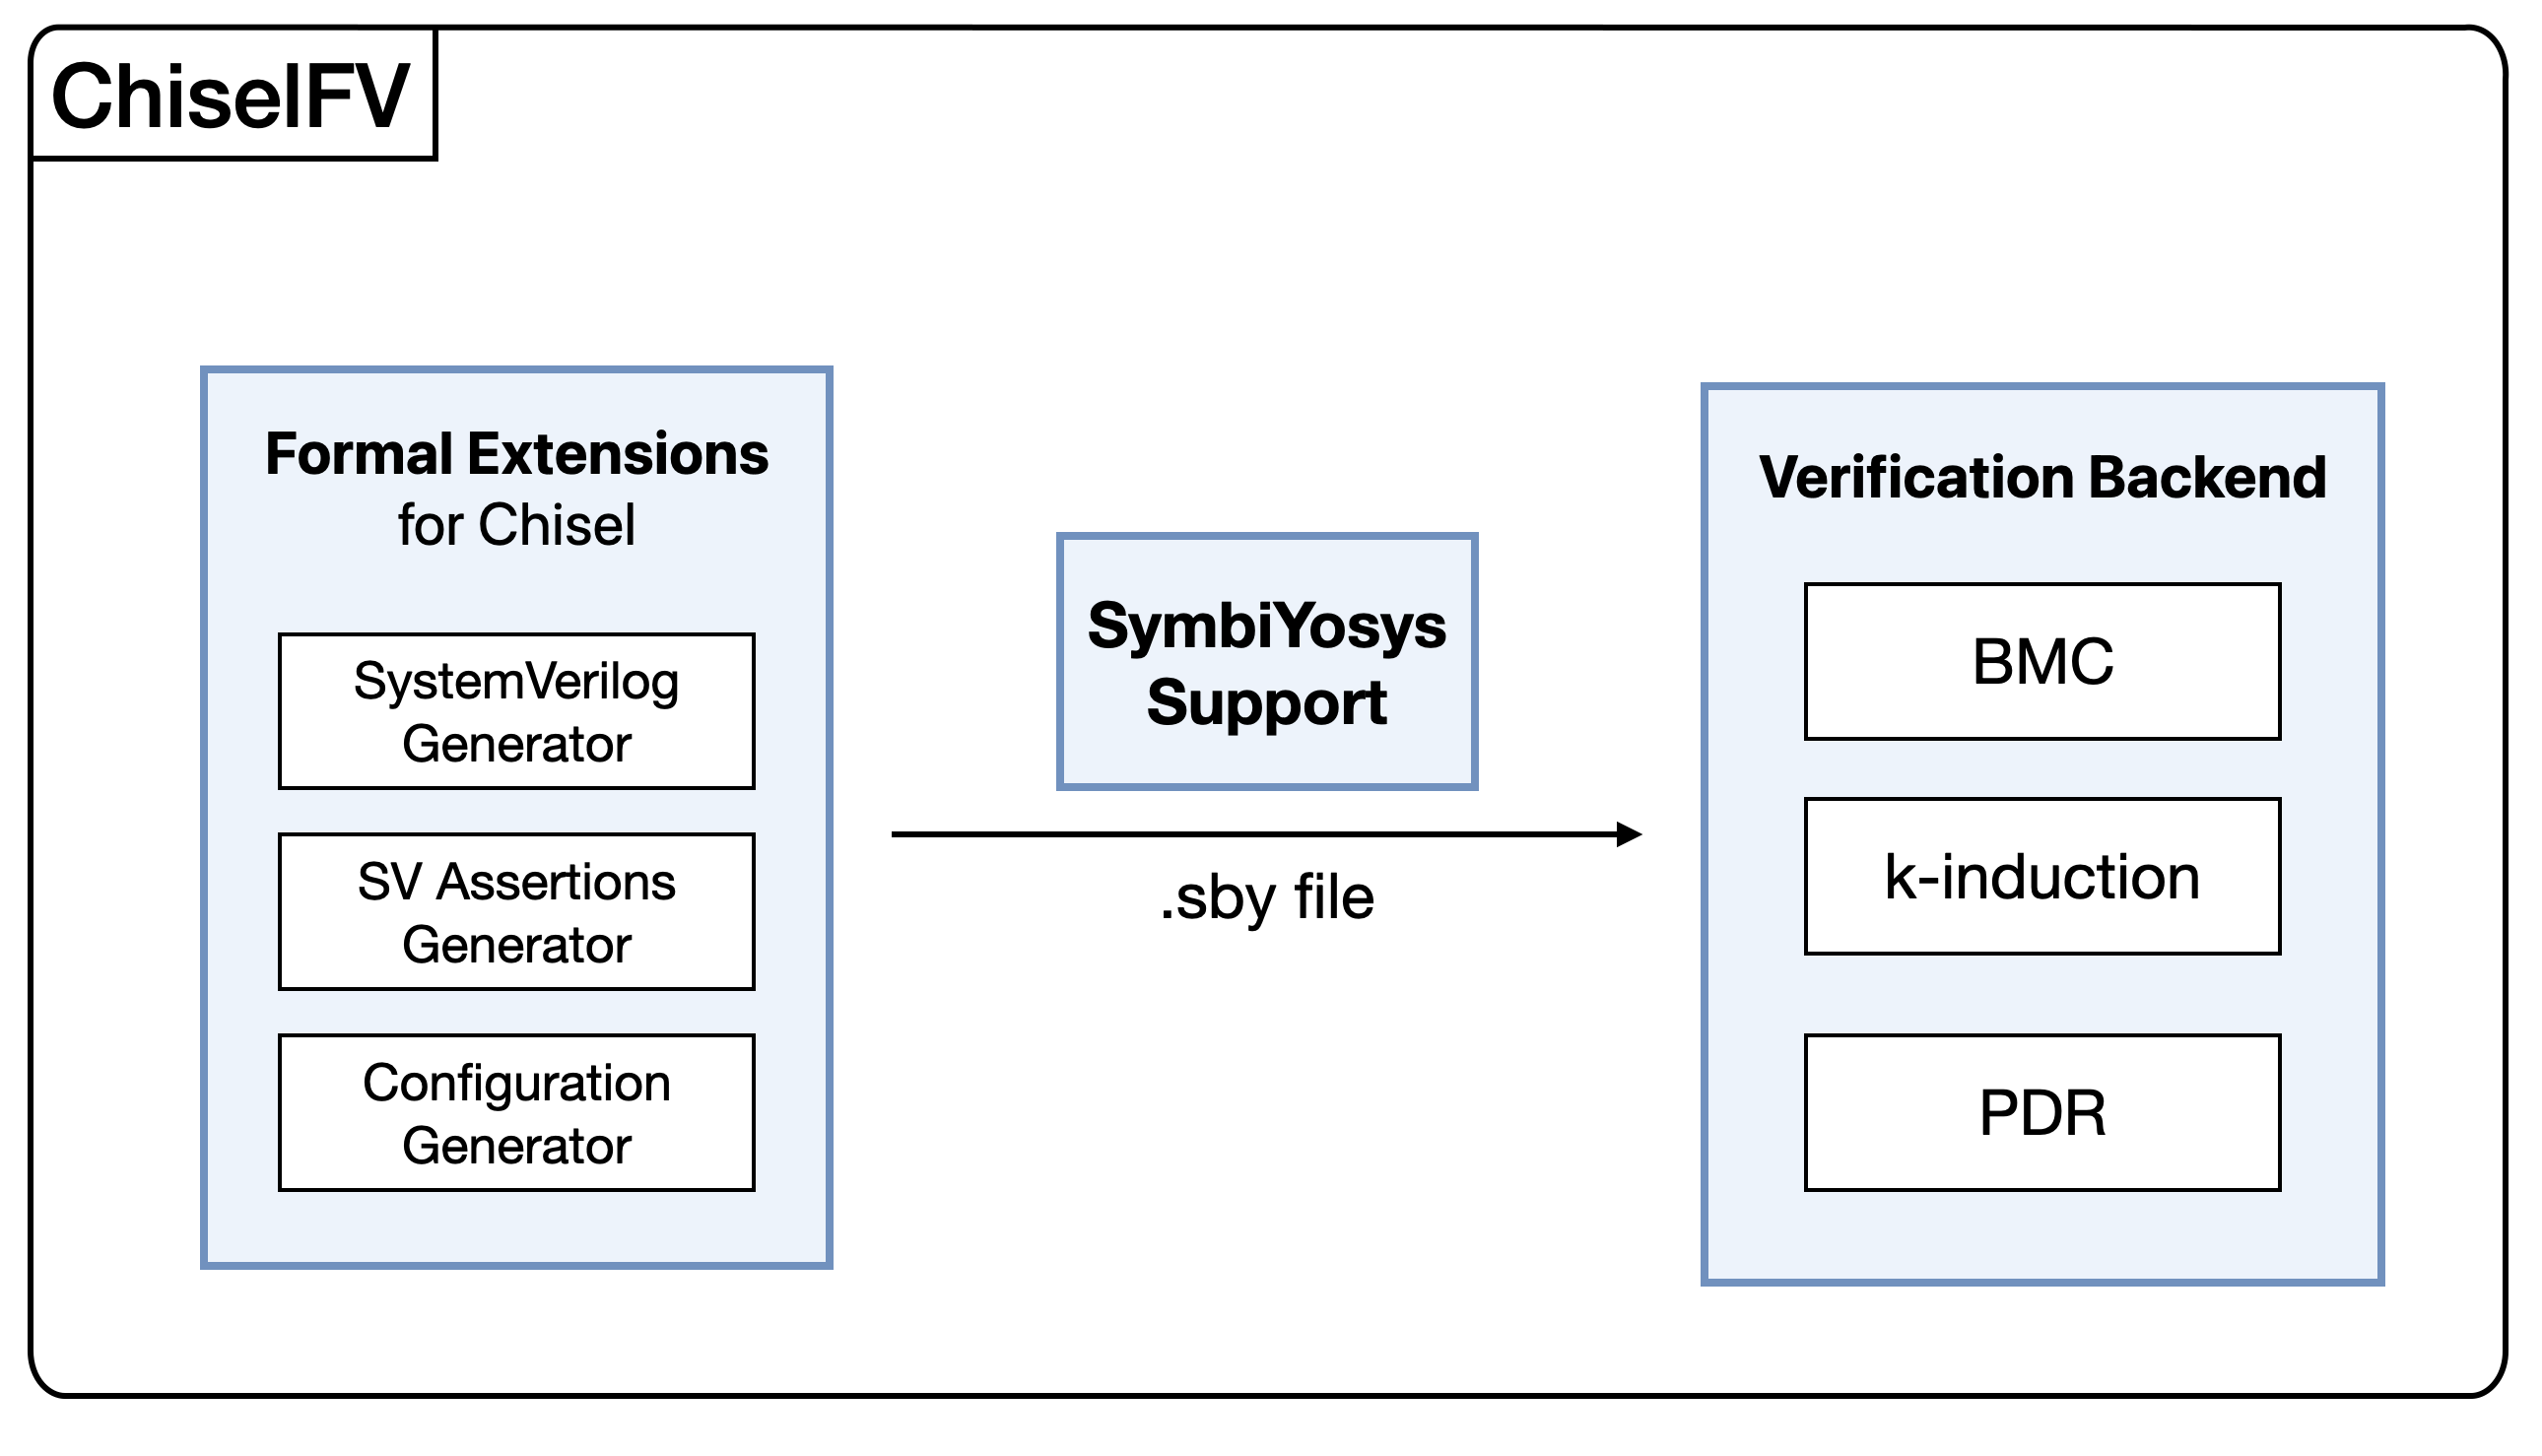
\includegraphics[width=1\linewidth]{pics/structure.png}
    \caption{ChiselFV Structure}
    \label{fig: structure}
    \end{center}
\end{figure}

As shown in Fig \ref{fig: structure}, ChiselFV is mainly an extension of Chisel's SystemVerilog generation and adds support for formal verification syntax. It also integrates the verification frontend and backend based on SymbiYosys, enabling one-key verification. The SystemVerilog generation is performed by calling the SystemVerilog generation process in Chisel. In contrast, for property descriptions, the compilation of the corresponding SystemVerilog Assertions (SVA) \cite{vijayaraghavan2005practical} script is performed, and some auxiliary circuits, in order to implement more complex property descriptions. And the configuration generator generates SymbiYosys-supported verification tasks configuration file .sby. 

\subsubsection{Formal Extensions For Chisel}

Hardware developers can construct hardware modules in Chisel and Chisel's compiler can compile Chisel modules to SystemVerilog code, and the starting point of our work is of injecting support for formal property descriptions in this stage.


% \begin{table}[htbp]
% \caption{Table Type Styles}
% \begin{center}
% \begin{tabular}{|c|c|c|c|}
% \hline
% \textbf{Table}&\multicolumn{3}{|c|}{\textbf{Table Column Head}} \\
% \cline{2-4} 
% \textbf{Head} & \textbf{\textit{Table column subhead}}& \textbf{\textit{Subhead}}& \textbf{\textit{Subhead}} \\
% \hline
% copy& More table copy$^{\mathrm{a}}$& &  \\
% \hline
% \multicolumn{4}{l}{$^{\mathrm{a}}$Sample of a Table footnote.}
% \end{tabular}
% \label{tab1}
% \end{center}
% \end{table}

% \begin{figure}[htbp]
% \centerline{\includegraphics{fig1.png}}
% \caption{Example of a figure caption.}
% \label{fig}
% \end{figure}


\bibliographystyle{IEEEtran}
\bibliography{./ref.bib}

\end{document}
